\documentclass[envcountsect, smaller, aspectratio=149]{beamer}
\usetheme[headheight=0em, logo=none, themepath=beamercolorthemefibeamer, nofonts]{fibeamer}
\usepackage{beamercolorthemefibeamer}
\setbeamerfont{frametitle}{size=\large}
\usepackage[utf8]{inputenc}
\usepackage[english, ngerman]{babel}
\usepackage{caption}
\usepackage{mathtools}
\usepackage{amsmath}
\usepackage{animate}
\usepackage{xmpmulti}
\usepackage{tikz}
\usepackage{multirow}
\usetikzlibrary{matrix}
\DeclareMathAlphabet{\mymathbb}{U}{BOONDOX-ds}{m}{n}


\makeatletter
\makeatother
\useoutertheme{infolines}
\newenvironment{noheadline}{
	\setbeamertemplate{headline}{}
}{}
\newenvironment{nofootline}{
\setbeamertemplate{footline}{}
}{}

\setbeamersize{text margin left=2.7em, text margin right=2.7em}
\setbeamertemplate{frametitle}{\insertframetitle}
\setbeamercolor{block body}{fg=black!90}

\setbeamerfont{title}{size=\huge}
\setbeamertemplate{institute}{\insertinstitute}

\AtBeginSection{
	\begin{noheadline}
		\begin{frame}
		\vfill
		\centering
		\begin{beamercolorbox}[sep=8pt,center]{title}
			\usebeamerfont{title}\insertsectionhead\par%
		\end{beamercolorbox}
		\vfill
	\end{frame}
	\end{noheadline}
}


\captionsetup{justification=centering}
\bibliographystyle{abbrv}

\newtheorem{proposition}{Proposition}
\setbeamertemplate{proof begin}{\vspace{0.5ex}%
{\emph{\insertproofname\ } }%
}
\setbeamertemplate{proof end}{\par
}

\newcommand{\diff}{\,\textrm{d}}
\newcommand{\R}{\mathbb{R}}
\newcommand{\N}{\mathbb{N}}
\newcommand{\Z}{\mathbb{Z}}
\newcommand{\norm}[1]{\left\lVert#1\right\rVert}
\newcommand{\abs}[1]{\left\lvert#1\right\rvert}
\newcommand{\avg}{\textnormal{avg}}

\newcommand{\todo}[1]{{\color{red} #1}}
%%%%%
%% MAYBE DO:
%% INFORMATIONAL APPROACH POOLING
%% CONVOLUTION WITH GROUP THEORY
%% PRACTICAL TEST CNNs
%% LAYER NUMBER l+1 vs l
%% FEHLERANFÄLLIGKEIT
%% INVARIANCE OF POOLING
%% BACKPROPAGATION CONV. NEURAL NETWORKS
%%%%%

\title{Neuronale Faltungsnetze und Pooling}
\author{Michael Markl}
\date{25. Juni 2021}
\subtitle{Mathematische Aspekte des Maschinellen Lernens\\
Seminar bei Prof. Dr. Stykel}
\begin{document}

\begin{nofootline}
    \frame{\titlepage}
\end{nofootline}

\begin{frame}{Experiment von Hubel und Wiesel~\cite{Hubel1959, Hubel1962}}
    
\begin{figure}
    \vspace*{-2em}
    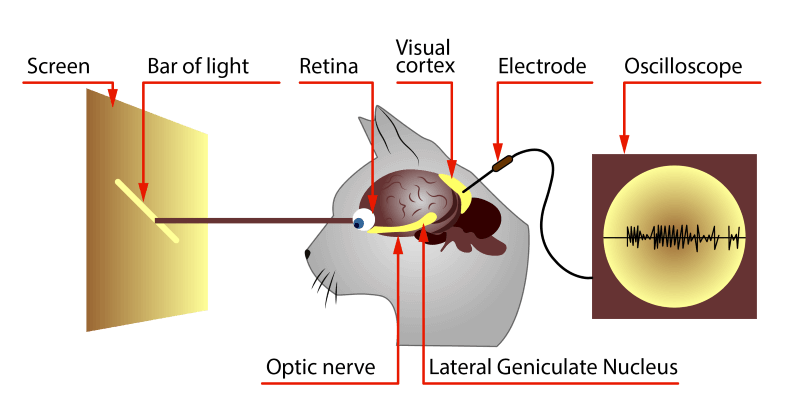
\includegraphics[width=0.8\textwidth]{../cat-experiment.png}
    \vspace{-1em}
    \caption{Messung der Aktivität einzelner Neuronen des visuellen Cortex bei Licht-Reizen. {\scriptsize(Grafik aus~\cite{Ver17})}}
\end{figure}

\end{frame}

\begin{frame}{Drei Kernresultate des Experiments}

\begin{minipage}[t]{1.05\textwidth}
    \begin{itemize}
    \onslide<2->\item Jedes Neuron hat ein \textbf{lokales rezeptives Feld},
        d.\,h. es reagiert nur auf Reize aus einer kleinen Umgebung des Ursprungsbildes.
    \onslide<3->{\item Auf dem rezeptiven Feld hat das Neuron \textbf{erregende} (engl. excitatory) \textbf{und} \textbf{hemmende} (engl. inhibitory) \textbf{Regionen}.}
    \onslide<4->{\item Der visuelle Cortex ist in Spalten aufgebaut.
    Neuronen \textbf{tieferer Schichten} nutzen als Rezeptoren die Aktivierung von Neuronen der Schicht darunter und erkennen \textbf{komplexere Strukturen}.}
\end{itemize}
\end{minipage}

\vspace{0.5em}
\begin{minipage}[c]{0.5\textwidth}
    \onslide<2->{
    \begin{figure}
        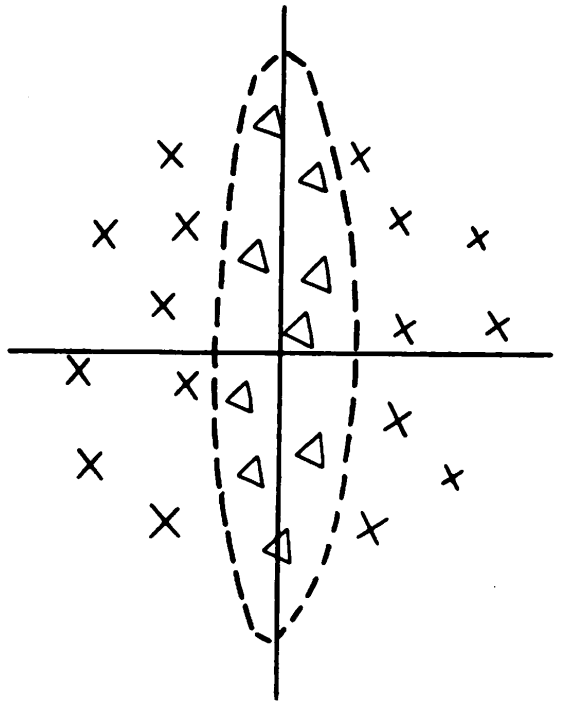
\includegraphics[width=0.35\textwidth]{../receptive-field-cat.png}
        \vspace{-0.5em}
        \caption{Rezeptives Feld eines Neurons.\\$x$: erregend; $\Delta$: hemmend. {\scriptsize (Grafik~aus~\cite{Hubel1959})}}
    \end{figure}
    }
\end{minipage}%
\begin{minipage}[c]{0.5\textwidth}
\onslide<4->{
    \begin{figure}
        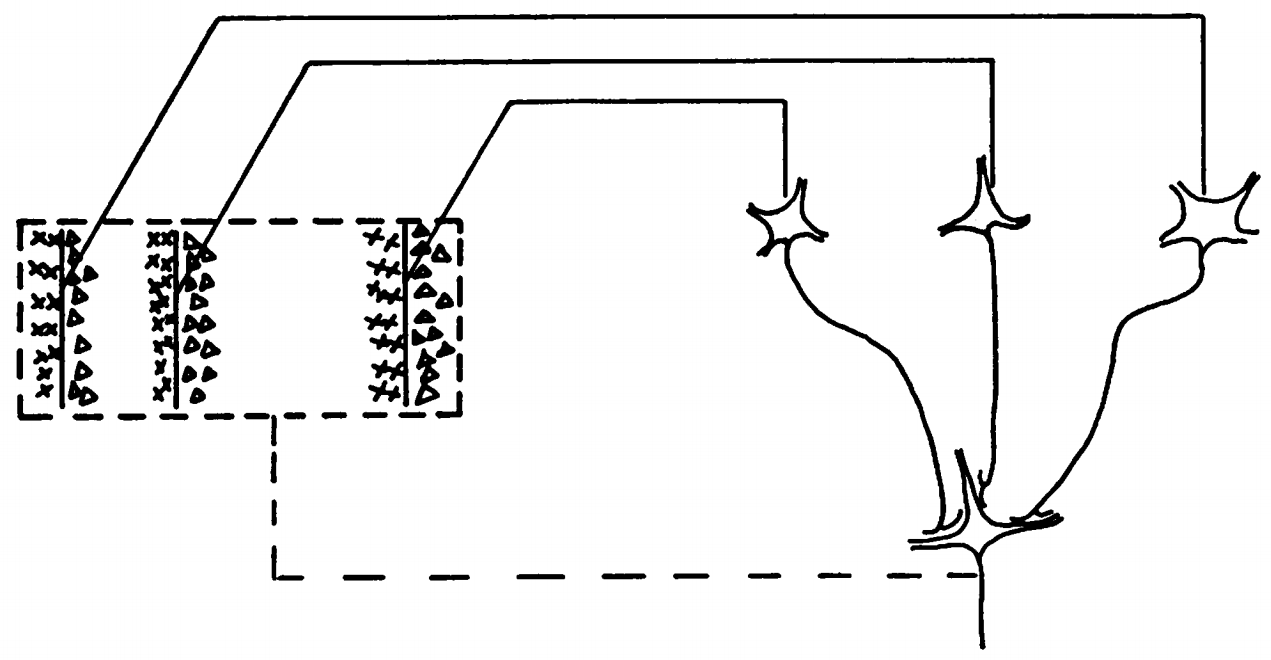
\includegraphics[width=0.86\textwidth]{../complex-cells.png}
        \vspace{-0.5em}
        \caption{Aufbau komplexer Zellen {\scriptsize (Grafik~aus~\cite{Hubel1962})}}
    \end{figure}
}
\end{minipage}
\end{frame}

%%%%
% Hubel und Wiesel haben dafür 1981 den Nobel-Preis erhalten.


\begin{frame}{Gliederung}
    \tableofcontents
\end{frame}



\section{Faltung und Kreuzkorrelation}
\subsection{Definition}
\begin{frame}[t]
    \begin{definition}[Kontinuierliche Signale]
        Ein kontinuierliches Signal $f:\R^d \rightarrow \R$
        \begin{itemize}            
            \item hat einen \emph{kompakten Träger}, falls $\exists R > 0: \norm{x}_\infty \geq R \implies f(x) = 0$,
            \item heißt  \emph{$L^1$-endlich}, falls $\norm{f}_1 \coloneqq \int_{\R^d} \abs{f(x)} \diff x < \infty$,
            \item heißt \emph{Energie-Signal}, falls $\norm{f}_2 \coloneqq \left(\int_{\R^d} f(x)^2 \diff x \right)^{1/2} < \infty$.
        \end{itemize}
    \end{definition}
    \pause
    \begin{proposition}
        Ein kontinuierliches Energie-Signal mit kompaktem Träger ist $L^1$-endlich.
    \end{proposition}
    \pause
    \begin{proof}
        Mit Cauchy-Schwarz-Ungleichung:
        \vspace{-0.5em}
        \begin{align*}
            \norm{f}_1^2 
            &= \int_{\R^d} \abs{f(x)} \cdot \mathbf{1}_{B_R(0)}(x) \diff x
            = \langle \abs{f}, \mathbf{1}_{B_R(0)} \rangle_{L_2}\\
            &\leq \norm{f}_2 \cdot \norm{ \mathbf{1}_{B_R(0)}}_2 < \infty
            \qedhere.
        \end{align*}
        \vspace{-1em}
    \end{proof}
\end{frame}


\begin{frame}[t]
    \begin{definition}[Diskrete Signale]
        Ein diskretes Signal $f:\Z^d \rightarrow \R$
        \begin{itemize}
            \item hat einen \emph{kompakten Träger}, falls $\exists R > 0: \norm{x}_\infty \geq R \implies f(x) = 0$,
            \item heißt  \emph{$L^1$-endlich}, falls $\norm{f}_1 \coloneqq \sum_{x\in\Z^d} \abs{f(x)} < \infty$,
            \item heißt \emph{Energie-Signal}, falls $\norm{f}_2 \coloneqq \left(\sum_{x\in\Z^d} f(x)^2 \right)^{1/2} < \infty$.
        \end{itemize}
    \end{definition}
    \pause \begin{proposition}
        Ein diskretes Signal mit kompaktem Träger ist $L^1$-endlich.
    \end{proposition}
\end{frame}



\begin{frame}[t]
    \begin{definition}[Kontinuierliche Faltung, Kreuzkorrelation]
        Die \emph{Faltung} (engl. \foreignlanguage{english}{convolution}) zweier kontinuierlicher Signale $f,g: \R^d \rightarrow \R$ bezeichnet
        \[
          (f*g) (x) \coloneqq \int_{\R^d} f(\tau) \cdot g(x-\tau) \diff \tau \quad\text{für $x\in \R^d$}.
        \]%
        Die \emph{Kreuzkorrelation} (engl. \foreignlanguage{english}{cross-correlation}) von $f$ und $g$ bezeichnet
        \[
            (f\star g) (x) \coloneqq \int_{\R^d} f(\tau) \cdot g(x+\tau) \diff \tau \quad\text{für $x\in \R^d$}.
        \]
        \pause
        In ML heißt $f$ der \emph{Kernel} oder \emph{Filter}, $g$ das \emph{Eingangssignal} 
        und $f\star g$ die \emph{Feature-Map}.
    \end{definition}
    
\end{frame}

\begin{frame}[t]
    \begin{definition}[Diskrete Faltung, Kreuzkorrelation]
        Die \emph{Faltung} (engl. \foreignlanguage{english}{convolution}) zweier diskreter Signale $f,g: \Z^d \rightarrow \R$ \\
        bezeichnet
        \[
          (f*g) (x) \coloneqq \sum_{\tau\in \Z^d} f(\tau) \cdot g(x-\tau) \quad\text{für $x\in \Z^d$}.
        \]%
        Die \emph{Kreuzkorrelation} (engl. \foreignlanguage{english}{cross-correlation}) von $f$ und $g$ bezeichnet
        \[
            (f\star g) (x) \coloneqq \sum_{\tau\in \Z^d} f(\tau) \cdot g(x+\tau) \quad\text{für $x\in \Z^d$}.
        \]
        In ML heißt $f$ der \emph{Kernel} oder \emph{Filter}, $g$ das \emph{Eingangssignal} 
        und $f\star g$ die \emph{Feature-Map}.
    \end{definition}
    \begin{itemize}
        \pause\item Es gilt $f\star g= (\tau\mapsto f(-\tau)) * g = \int f(\tau - x) \cdot g(\tau) \diff \mu(\tau)$.
        \pause\item Faltung ist kommutativ, assoziativ und distributiv über $+$.
        \pause\item Bei neuronalen Faltungsnetzen wird mit Faltung meist Kreuzkorrelation gemeint.
    \end{itemize}
\end{frame}

\subsection{Beispiele}

\begin{frame}{Beispiele im Eindimensionalen}
    \begin{itemize}
        \item Rechteck- und Dreieckssignal\\
        {
        \centering
        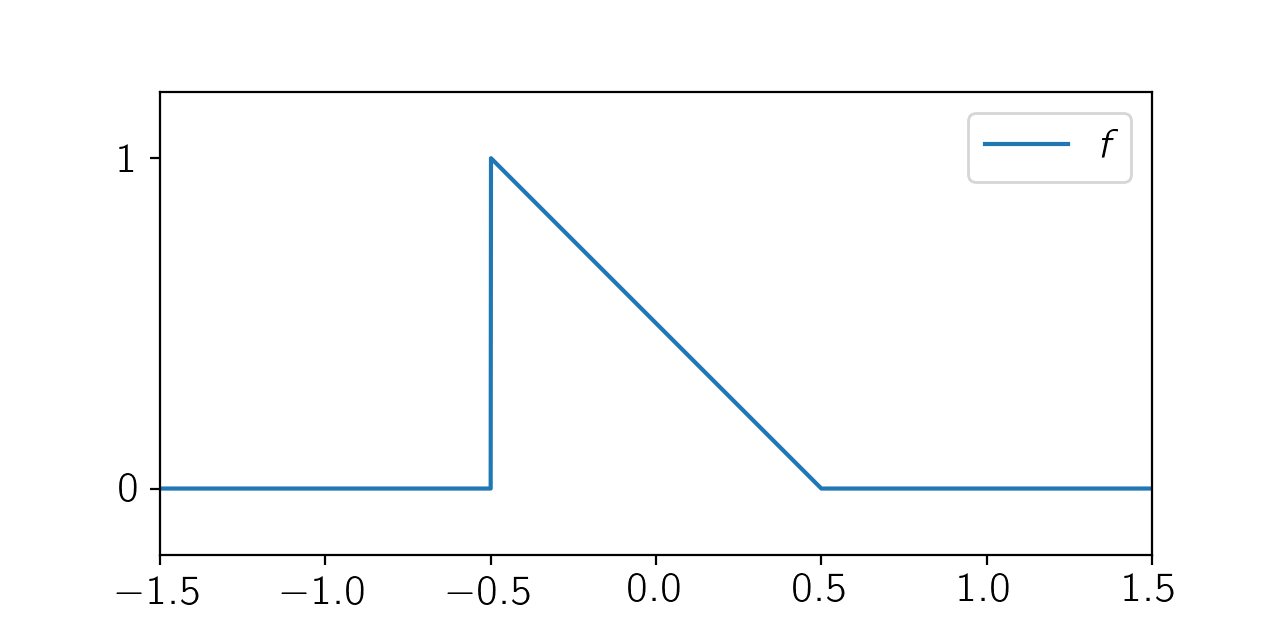
\includegraphics[width=0.45\textwidth]{../f.png}
        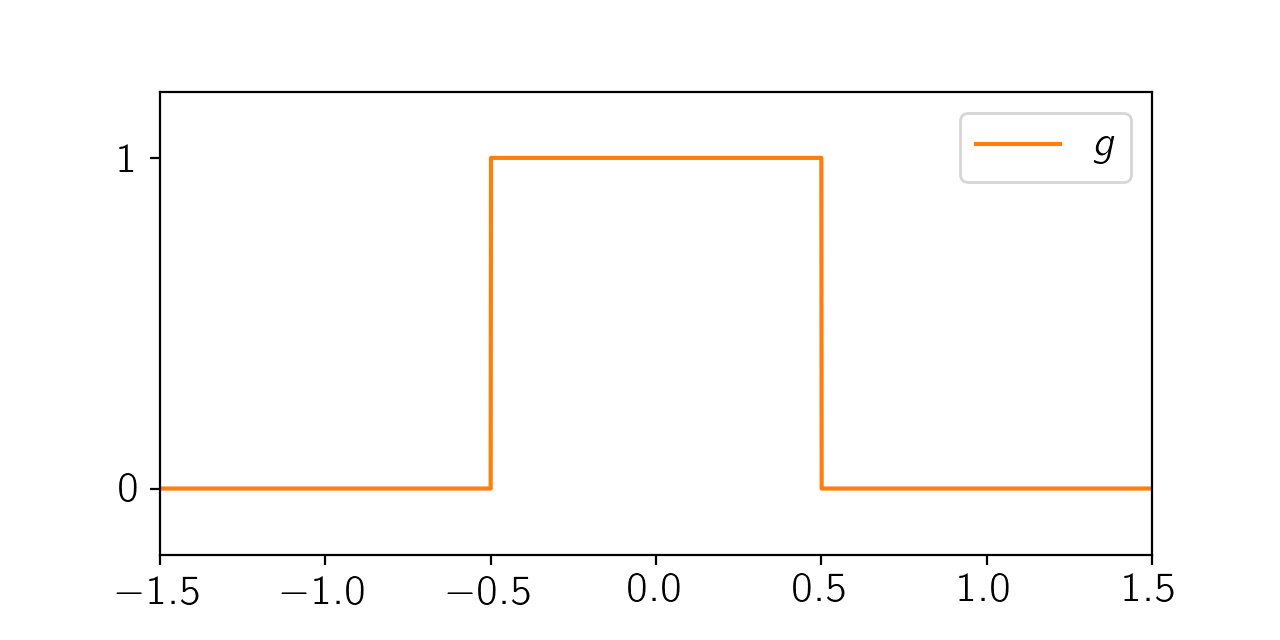
\includegraphics[width=0.45\textwidth]{../g.png}
        }
        \pause
        \item Mit $f = (\dots, 0, 0, f_0 = \frac{1}{2}, f_1 = \frac{1}{2}, 0, 0, \dots)$ ergibt 
        $f \star g$
        den \emph{gleitenden Mittelwert von $g$}: \[(f\star g)_i = f_0 \cdot g_i + f_1 \cdot g_{i + 1} = \frac{g_i + g_{i+1}}{2}\]
    \end{itemize}
\end{frame}

\begin{frame}{Beispiele im Zweidimensionalem}
\begin{itemize}
    \item Graustufen-Bilder werden bspw. enkodiert als $X\in[0,1]^{M_1\times N_1}$ mit $0\, \hat= \,\text{schwarz}$ und $1\,\hat{=}\,\text{weiß}$.
\end{itemize}
\begin{center}
\begin{minipage}[t]{0.3\textwidth}
    \centering
    Input $X\in [0,1]^{28x28}$:
    \begin{figure}
        
\includegraphics[width=\textwidth]{4.png}
    \end{figure}
\end{minipage}
\begin{minipage}[t]{0.3\textwidth}
    \centering
    Kernel $W$:
    \vspace{0.25\textwidth}
    \[
        \left(\begin{array}{ccc}
            \frac{1}{4} & \frac{1}{2} & \frac{1}{4} \\[4pt]
            0 & 0 & 0 \\[4pt]
            -\frac{1}{4} & -\frac{1}{2} & -\frac{1}{4}
        \end{array}\right)
    \]
\end{minipage}
\begin{minipage}[t]{0.3\textwidth}
    \centering
    Kreuzkorrelation $W\star X$:
    \begin{figure}
        \vspace{0.0357\textwidth}
        
\includegraphics[width=0.9285\textwidth]{4-convolved.png}
    \end{figure}
\end{minipage}
\end{center}
\end{frame}

%%%%%%%%
% CROSS-CORRELATION GIBT DIE ÄHNLICHKEIT ZWEIER SIGNALE IN ABHÄNGIGKEIT DER VERZÖGERUNG
% ZWISCHEN DEN SIGNALEN AN.
% CONVOLUTION HINGEGEN SPIEGELT DIE ANTWORT EINES SIGNALS AUF EINEN FILTER WIDER.
%%%%%%%%

\newcommand{\transl}[2]{T_{#1}\, #2}
\subsection{Eigenschaften der Faltung}
\begin{frame}
    \begin{proposition}
        Sind $f$ und $g$ $L^1$-endliche Signale, so auch $f\star g$.
    \end{proposition}
    \pause
    \begin{proof}
        Wir nutzen den Satz von Fubini:
        \begin{align*}
            \norm{f \star g}_1
            &= \int_{\R^d} \abs{ \int_{\R^d} f(\tau)\cdot g(x + \tau) \diff\tau }\diff x
            \leq \int_{\R^d}  \int_{\R^d} \abs{f(\tau)\cdot g(x + \tau)} \diff\tau \diff x\\
            &= \int_{\R^d} \abs{f(\tau)} \cdot \int_{\R^d} \abs{g(x+\tau)} \diff x \diff\tau
            = \norm{f}_1 \cdot \norm{g}_1 \qedhere.
        \end{align*}
    \end{proof}
    \pause
    \begin{proposition}[Äquivarianz bzgl. Translation]
        Sei $\mathcal{C}(g)\coloneqq f\star g$ und $(\transl{a}{g})(x) \coloneqq g(x - a)$ für ein Signal $f$ und $a\in\R^d$.
        Dann gilt \[ \mathcal{C}(\transl{a}{g}) = \transl{a}{\mathcal{C}(g)}. \]
    \end{proposition}
    \pause
    \begin{proof}
        $\mathcal{C}(T_a\, g)(x) = \int_{\R^d} f(\tau) \cdot g(x - a + \tau) \diff \tau = \transl{a}{\mathcal{C}(g)}$
    \end{proof}
\end{frame}


\section{Faltungslayer}

\subsection{Faltungslayer mit eindimensionalem Input}

\begin{frame}{Faltungslayer mit eindimensionalem Input}
\begin{minipage}{0.60\textwidth}
    \begin{itemize}
        \onslide<+->{\item Bei ML-Anwendungen werden meist nur Eingangssignale $x$ und Kernel $w$ mit kompaktem Träger betrachtet.}
        \onslide<+->{\item Hier: $x=(x_0, \dots, x_{n-1})$, $w=(w_0,\dots, w_{m-1})$ mit $n\geq m$.}
        \onslide<+->{\item Der Output $y$ eines Faltungslayers mit Kernel $w$ kann beschrieben werden durch \[
            y_i = \sigma( (w \star x)_i + b ) = \sigma\left( \sum_j w_j \cdot x_{i+j} + b \right).
            \]}
        \onslide<+->{\item Die Einträge des Kernel sowie das Skalar $b$ sind die zu lernenden Parameter.}
        \onslide<+->{\item Ein Layer verwendet meist mehrere Kernel $(w^i)_{i=1,\dots,f}$ parallel.}
    \end{itemize}
\end{minipage}\hfill
\begin{minipage}{0.35\textwidth}
    \onslide<2->{
    \centering
    \begin{figure}
        \begin{tikzpicture}[main/.style = {draw, outer sep=3pt}] 
    \node[main] (x0) at (0, 0)  {$x_0$}; 
    \node[main] (x1) at (0, -1) {$x_1$};
    \node[main] (x2) at (0, -2) {$x_2$}; 
    \node[main] (x3) at (0, -3) {$x_3$};
    \node[main] (x4) at (0, -4) {$x_4$}; 
    \node[main] (x5) at (0, -5) {$x_5$};

    \node (y0) at (2, -0.5) {$\sigma$};
    \node (y1) at (2, -1.5) {$\sigma$};
    \node (y2) at (2, -2.5) {$\sigma$};
    \node (y3) at (2, -3.5) {$\sigma$};
    \node (y4) at (2, -4.5) {$\sigma$};

    \node[main] (yy0) at (3, -0.5) {$y_0$};
    \node[main] (yy1) at (3, -1.5) {$y_1$};
    \node[main] (yy2) at (3, -2.5) {$y_2$};
    \node[main] (yy3) at (3, -3.5) {$y_3$};
    \node[main] (yy4) at (3, -4.5) {$y_4$};

    \draw [->] (x0) -> node[above, align=center] {$w_0$} (y0);
    \draw [->] (x1) -> node[above, align=center] {$w_1$} (y0);
    \draw [->, gray] (y0) + (0,0.5) -> node[above=3pt, align=center, black] {$b$} (y0);
    \draw [->] (y0) -> (yy0);

    \draw [->] (x1) -> node[above, align=center] {$w_0$} (y1);
    \draw [->] (x2) -> node[above, align=center] {$w_1$} (y1);
    \draw [->, gray] (y1) + (0,0.5) -> node[above=1pt, align=center] {} (y1);
    \draw [->] (y1) -> (yy1);


    \draw [->] (x2) -> node[above, align=center] {$w_0$} (y2);
    \draw [->] (x3) -> node[above, align=center] {$w_1$} (y2);
    \draw [->, gray] (y2) + (0,0.5) -> node[above=1pt, align=center] {} (y2);
    \draw [->] (y2) -> (yy2);


    \draw [->] (x3) -> node[above, align=center] {$w_0$} (y3);
    \draw [->] (x4) -> node[above, align=center] {$w_1$} (y3);
    \draw [->, gray] (y3) + (0,0.5) -> node[above=1pt, align=center] {} (y3);
    \draw [->] (y3) -> (yy3);


    \draw [->] (x4) -> node[above, align=center] {$w_0$} (y4);
    \draw [->] (x5) -> node[above, align=center] {$w_1$} (y4);
    \draw [->, gray] (y4) + (0,0.5) -> node[above=1pt, align=center] {} (y4);
    \draw [->] (y4) -> (yy4);

\end{tikzpicture} 

        \caption{Eindim. Faltungslayer mit $n=5,m=2$.}
    \end{figure}
    }
\end{minipage}
\end{frame}

\begin{frame}
    \begin{definition}[Eindimensionales Faltungslayer]
        Ein eindimensionales Faltungslayer hat die folgenden Eigenschaften:
        \begin{itemize}
            \item die räumliche Input-Größe $d^{(l)}$,
            \item die räumliche Kernel-Größe $m^{(l)}$,
            \item die Anzahl an Input-Feature-Maps $f^{(l)}$,
            \item die Anzahl an Output-Feature-Maps $f^{(l+1)}$,
            \item die Aktivierungsfunktion $\sigma^{(l)}$.
        \end{itemize}

        \pause Inputs des Layers haben die Form $x^{(l)}\in\R^{d^{(l)} \times f^{(l)}}$.\\[.4em]

        \pause Es werden $f^{(l+1)}$ Kernels und Biases der Form $w^{(l),k}\in\R^{m^{(l)} \times f^{(l)}}, b^{(l),k}\in\R$ für  $k\in\{0,\dots, f^{(l+1)}-1\}$ gelernt.\\[.4em]

        \pause Die räumliche Output-Größe ist $d^{(l+1)} = d^{(l)}-  m^{(l)} + 1$.\\[.4em]

        \pause Outputs des Layers haben die Form $x^{(l+1)}\in \R^{d^{(l+1)}\times f^{(l+1)}}$ und es gilt
        \[
            x^{(l+1)}_{i,k} =  \sigma^{(l)}\left( (w^{(l),k} \star x^{(l)})_{i} + b^{(l),k} \right)
        \]
    \end{definition}
\end{frame}

\begin{frame}{Faltungslayer mit eindimensionalem Input}
    Sind $x\in\R^n, w\in\R^m$, lässt sich der Ausdruck  \[
        y_i = \sigma( (w \star x)_i + b ) = \sigma\left( \sum_j w_j \cdot x_{i+j} + b \right)
    \]
    auch in die Matrixform $y = \sigma(Wx + B)$ bringen.
    Dabei ist $B=(b,\dots,b)^T$ und (am Beispiel $n=6,m=2$)
    \[
        W = \left(
      \begin{array}{cccccccccc}
        w_0 & w_1 & 0 & 0 & 0 & 0  \\
        0 & w_0 & w_1 & 0 & 0 & 0  \\
        0 & 0 & w_0 & w_1 & 0 & 0  \\
        0 & 0 & 0 & w_0 & w_1 & 0  \\
        0 & 0 & 0 & 0 & w_0 & w_1  \\
      \end{array} \right) .
    \]
    Eine Matrix dieser Form nennt man \emph{Toeplitz-Matrix}.
\end{frame}

%%%%%%%%%%
% DA DIE EINTRÄGE DES KERNEL ALS GEWICHTE GELERNT WERDEN,
% IST ES PRINZIPIELL EGAL, OB MAN ECHTE FALTUNG ODER CROSS-CORRELATION NUTZT.
% NUTZT MAN CONVOLUTION, WIRD EBEN EIN GEFLIPPTER KERNEL GELERNT;
% FÜR DIE IMPLEMENTIERUNG IST ES ABER EINFACHER CROSS-CORRELATION ZU VERWENDEN:
% DIE GÜLTIGEN, ZU BETRACHTENDEN INDIZES SIND SO EINFACHER ZU BESTIMMEN.
%%%%%%%%%%

\begin{frame}
    \begin{theorem}[Komposition von eindimensionalen Faltungslayern]
        Seien $w^{(1)}\in\R^{m^{(1)}}, w^{(2)}\in\R^{m^{(2)}}, \dots, w^{(L)}\in\R^{m^{(L)}}$ die (einzigen) Kernel von in Reihe geschalteten eindimensionalen Faltungslayern mit Biases $b^{(1)},\dots, b^{(L)}\in\R$ und linearer Aktivierungsfunktionen $\sigma^{(l)}(x) \coloneqq x$ für $l\in\{1,\dots,L\}$.

        Dann gibt es ein äquivalentes Netz mit nur einem Faltungslayer mit linearer Aktivierungsfunktion und Kernel $w\in\R^m$ mit $m=\sum_{i=1}^L m_i - (L-1)$.
    \end{theorem}

    %%%%%%%%%%
    % WAS HEIẞT ÄQUIVALENT? DAS HEIẞT, DASS DAS NETZWERK JEDEN INPUT
    % DEN SELBEN OUTPUT ZUWEIST.  
    %%%%%%%%%%

    \begin{proof}
        \pause Es genügt, die Aussage für $L=2$ zu zeigen; der Rest folgt per Induktion über $L$:
        \begin{itemize}
            \pause \item Der Induktionsanfang bei $L=1$ gilt trivialerweise.
            \pause \item Induktionsschritt \glqq$L\Rightarrow L+1$\grqq:
            
            Nach I.\,V. können die ersten $L$ Layer zu einem äquivalenten Faltungslayer mit Kernel $w'\in \R^{m'}$ mit $m'=\sum_{i=1}^L m_i - (L-1)$ überführt werden.

            \pause Fusionieren dieses Layers mit dem $(L+1)$-ten Layer ergibt ein äquivalentes Faltungslayer mit einem Kernel $w\in\R^m$ mit \[
                m = m' + m^{(L+1)} - (2-1) \pause = \sum_{i=1}^L m^{(i)} - (L-1) + m^{(L+1)} - 1 \pause = \sum_{i=1}^{L+1} m^{(i)} - (L+1 - 1)
                \]
        \end{itemize}
        \renewcommand{\qedsymbol}{}
    \end{proof}
\end{frame}

\begin{frame}
    \begin{proof}[Beweis für $L=2$]
        Seien $\alpha\in\R^k$, $b_1\in\R$ und $\beta\in\R^l$, $b_2\in\R$ die Kernel und Biases des ersten bzw. zweiten Faltungslayers.

        \pause Die erzeugten Toeplitz-Matrizen haben die Form
        \setlength\arraycolsep{2pt}
        \def\arraystretch{0.5}
        \[
            \mathcal{A} = \left(
                \begin{matrix}
                    \alpha_0 & \cdots & \alpha_{k-1} & 0 & \cdots & 0 \\
                    0 & \ddots & & \ddots  & & \vdots \\
                    \vdots  & & \ddots & & \ddots & 0 \\[4pt]
                     0 & \cdots & 0 & \alpha_0 & \cdots & \alpha_{k-1}
                \end{matrix}
            \right),\quad
            \mathcal{B} = \left(
                \begin{matrix}
                    \beta_0 & \cdots & \beta_{l-1} & 0 & \cdots & 0 \\
                    0 & \ddots & & \ddots  & & \vdots \\
                    \vdots  & & \ddots & & \ddots & 0 \\[4pt]
                     0 & \cdots & 0 & \beta_0 & \cdots & \beta_{l-1}
                \end{matrix}
            \right),
        \]
        mit $\mathcal{A}\in\R^{n - k + 1\times n}$ und $\mathcal{B}\in \R^{n-k-l+2 \times n-k+1}$.

        \pause Der Output des gemeinsamen Netzwerks ist:
        \[
            \mathcal{B}\cdot \left( \mathcal{A}\cdot x + B_1 \right) + B_2
            = \mathcal{B}\cdot \mathcal{A}\cdot x + \mathcal{B}\cdot B_1 + B_2.
        \]

        \pause Es gilt $(\mathcal{B}\cdot B_1 + B_2)_i = \sum_{j=0}^{l-1} \beta_j\cdot b_1 + b_2 \eqqcolon b$ für alle $i$.
        
        \pause Es bleibt zu zeigen, dass $\mathcal{B}\cdot \mathcal{A}$ die von einem Kernel der Länge $m\coloneqq k+l-1$ erzeugte Toeplitz-Matrix ist. 

        \renewcommand{\qedsymbol}{}
    \end{proof}
\end{frame}

\begin{frame}
    \setbeamertemplate{proof begin}{\vspace{0.5ex}%
{}%
}
\setbeamertemplate{proof end}{\par
}
    \begin{proof}
        Die erzeugten Toeplitz-Matrizen haben die Form
        \setlength\arraycolsep{2pt}
        \def\arraystretch{0.5}
        \[
            \mathcal{A} = \left(
                \begin{matrix}
                    \alpha_0 & \cdots & \alpha_{k-1} & 0 & \cdots & 0 \\
                    0 & \ddots & & \ddots  & & \vdots \\
                    \vdots  & & \ddots & & \ddots & 0 \\[4pt]
                     0 & \cdots & 0 & \alpha_0 & \cdots & \alpha_{k-1}
                \end{matrix}
            \right),\quad
            \mathcal{B} = \left(
                \begin{matrix}
                    \beta_0 & \cdots & \beta_{l-1} & 0 & \cdots & 0 \\
                    0 & \ddots & & \ddots  & & \vdots \\
                    \vdots  & & \ddots & & \ddots & 0 \\[4pt]
                     0 & \cdots & 0 & \beta_0 & \cdots & \beta_{l-1}
                \end{matrix}
            \right),
        \]
        mit $\mathcal{A}\in\R^{n - k + 1\times n}$ und $\mathcal{B}\in \R^{n-k-l+2 \times n-k+1}$.
        Sei $m\coloneqq k+l-1$.
        Es gilt
        \[
            \begin{aligned}
            (\mathcal{B} \cdot \mathcal{A})_i
            \pause &= \left(
                \begin{matrix}
                    \smash[b]{\underbrace{\begin{matrix}0 & \cdots & 0\end{matrix}}_{i-1}} & \beta_0 & \beta_1 & \cdots & \beta_{l-1} & 0 & \cdots & 0
                \end{matrix}
            \right) \cdot \mathcal{A} \\           
            \pause &= \left(
                    \begin{matrix}
                        \beta_0 & \beta_1 & \cdots & \beta_{l-1}
                    \end{matrix}
                \right) \cdot \left(\begin{matrix}
                    \mymathbb{0}_{l\times (i-1)} & \smash[b]{\underbrace{\begin{matrix}
                        \alpha_0 & \cdots & \alpha_{k-1} & 0 & \cdots & 0 \\
                        0 & \ddots & & \ddots  & & \vdots \\
                        \vdots  & & \ddots & & \ddots & 0 \\[4pt]
                        0 & \cdots & 0 & \alpha_0 & \cdots & \alpha_{k-1} \\
                \end{matrix}}_{l + k - 1 = m}} & \mymathbb{0}_{l\times (\geq 0)}\\[2em]
            \end{matrix}\right) \\[2em]
            \pause &= \left(\begin{matrix}
                \smash[b]{\underbrace{\begin{matrix}0 & \cdots & 0\end{matrix}}_{i-1}} &
                \smash[b]{\underbrace{\begin{matrix}\beta_0 \alpha_0 & ~\beta_0 \alpha_1 + \beta_1\alpha_0~ & \cdots & \sum_{j=0}^{l - 1} \beta_j \alpha_{m-1 - j}\end{matrix}}_{= \beta * \alpha \coloneqq w \text{ erzeugender Kernel}}} & 0 & \cdots & 0
            \end{matrix}\right).
        \end{aligned}
        \]
    \end{proof}
\end{frame}

\begin{frame}[t]{Anmerkungen}
    \begin{itemize}
        \pause \item Es ist wenig hilfreich, mehrere Faltungslayer mit linearer Aktivierungsfunktion in Reihe zu schalten.
        \pause \item Beim Fusionieren von zwei Faltungslayern mit den Kernel $\alpha$ und $\beta$, erhält man einen Faltungslayer mit Kernel $\alpha *\beta$. \pause Allgemeiner:
    \end{itemize}
    \begin{proposition}
        Für $L^1$-endliche Signale $f,g,h$ gilt $f\star (g \star h) = (f*g)\star h$.
    \end{proposition}
    \pause \begin{proof}
        Mit dem Satz von Fubini gilt
        \[
            \begin{aligned}
            (f\star (g\star h))(x)
            \pause &= \int_{\R^d} f(\tau) \cdot \int_{\R^d} g(\tau') \cdot h(x+\tau+\tau')\diff \tau' \diff \tau \\
            \pause &= \int_{\R^d} \int_{\R^d} f(\tau) \cdot g(\tau' - \tau)\cdot h(x+\tau')\diff \tau' \diff \tau \\
            \pause &= \int_{\R^d}\int_{\R^d} f(\tau) \cdot g(\tau'-\tau) \diff\tau \cdot h(x+\tau')\diff\tau' \\
            \pause &= \int_{\R^d}  (f * g)(\tau')\cdot h(x+\tau') \diff \tau'
            \pause = \left( (f * g) \star h \right)(x).
            \qedhere
            \end{aligned}
        \]
    \end{proof}
\end{frame}


\subsection{Faltungslayer mit zweidimensionalem Input}

\begin{frame}{Faltungslayer mit zweidimensionalem Input}
    \begin{itemize}
        \item Im zweidimensionalen Fall haben Input-Daten eines Netzwerks im Fall von Graustufen-Bildern mit Höhe $r$ und Breite $c$ meist die Form $x\in[0,1]^{r\times c\times 1}$.
        \item Für farbige Bilder gibt es meist $3$ verschiedene Channels für die Farben rot, grün und blau.
        Dementsprechend gilt $f^{(1)} = 3$ und $x^{(1)}\in[0,1]^{r\times c \times 3}$.
        \item Für zweidimensionale Faltungslayer ergibt sich für eine Output-Feature-Map anhand des Kernels $w\in\R^{m_r\times m_c\times f}$ mit Bias $b\in\R$
        \[
            y_{i, j} = \sigma( (w \star x)_{i,j,0} + b ) = \sigma\left( \sum_{p=0}^{m_r - 1} \sum_{q=0}^{m_c - 1} \sum_{k=0}^{f-1} w_{p,q,k} \cdot x_{i+p, j+q,k} + b \right).
        \]
    \end{itemize}
\end{frame}


\begin{frame}
    \begin{definition}[Zweidimensionales Faltungslayer]
        Ein zweidimensionales Faltungslayer hat die folgenden Eigenschaften:
        \begin{itemize}
            \item die räumliche Input-Größe $r^{(l)}\times c^{(l)}$,
            \item die räumliche Kernel-Größe $m_r^{(l)}\times m_c^{(l)}$,
            \item die Anzahl an Input-Feature-Maps $f^{(l)}$,
            \item die Anzahl an Output-Feature-Maps $f^{(l+1)}$,
            \item die Aktivierungsfunktion $\sigma^{(l)}$.
        \end{itemize}

        Inputs des Layers haben die Form $x^{(l)}\in\R^{m_r^{(l)}\times m_c^{(l)} \times f^{(l)}}$.\\[.4em]

        Es werden $f^{(l+1)}$ Kernels und Biases der Form $w^{(l),j}\in\R^{m_r^{(l)} \times m_c^{(l)} \times f^{(l)}}, b^{(l),j}\in\R$ für  $j\in\{1,\dots, f^{(l+1)}\}$ gelernt.\\[.4em]

        Die räumliche Output-Größe ist $r^{(l+1)} \times c^{(l+1)} = (r^{(l)}-  m_r^{(l)} + 1) \times (c^{(l)}-  m_c^{(l)} + 1) $.\\[.4em]

        Outputs des Layers haben die Form $x^{(l+1)}\in \R^{r^{(l+1)}\times c^{(l+1)} \times f^{(l+1)}}$ und es gilt
        \[
            x^{(l+1)}_{i,j,k} =  \sigma^{(l)}\left( (w^{(l),j} \star x^{(l)})_{i,j,0} + b^{(l),k} \right)
        \]
    \end{definition}
\end{frame}

\begin{frame}{Varianten bei Faltungslayern}
    In der Praxis werden oft Varianten der Kreuzkorrelation verwendet:
    \begin{itemize}
        \item Die \emph{Schrittbreite} $s\in\N$ (engl. \foreignlanguage{english}{stride}) bestimmt, wie viele Pixel der Kernel pro Schritt bewegt werden soll.
        Für $s=2$ ergibt sich:
        \begin{figure}
            \centering
            \includegraphics[width=0.17\textwidth]{no_padding_strides_00.pdf}
            \includegraphics[width=0.17\textwidth]{no_padding_strides_01.pdf}
            \includegraphics[width=0.17\textwidth]{no_padding_strides_02.pdf}
            \includegraphics[width=0.17\textwidth]{no_padding_strides_03.pdf}
        \end{figure}
        \item Es kann zusätzliches \emph{Padding} verwendet werden, sodass auch Teilüberdeckungen des Kernel mit dem Input erlaubt werden:
        \begin{figure}
            \centering
            \includegraphics[width=0.2\textwidth]{full_padding_no_strides_00.pdf}
            \includegraphics[width=0.2\textwidth]{full_padding_no_strides_01.pdf}
            \includegraphics[width=0.2\textwidth]{full_padding_no_strides_02.pdf}
            \includegraphics[width=0.2\textwidth]{full_padding_no_strides_03.pdf}
        \end{figure}

        \begin{center}
            \scriptsize (Grafiken aus~\cite{dumoulin2016guide})
        \end{center}
    \end{itemize}
\end{frame}




\section{Pooling}

\begin{frame}{Motivation für Pooling-Layer}
    \begin{itemize}
        \pause \item Viele Anwendungsfälle haben hochaufgelöste Input-Daten.
        \pause \item Mit Faltungslayern werden Features aus diesen Daten extrahiert; dabei wird die Auflösung meist nicht reduziert.
        \pause \item Bei Klassifizierungsaufgaben sind hohe Dimensionen problematisch: \\
        Ein Fully-Connected-Layer, das ein $100x100$ Bild mit $100$ Feature-Maps $x\in\R^{100\times 100\times 100}$ einer von $1000$ Kategorien zuweist, erzeugt eine Gewichtematrix mit $10^{9}$ Einträgen.\\
        $\implies$ Das ist speicher- und rechenaufwändig.
        \pause \item Stattdessen wird meist sukzessive die räumliche Dimension durch Pooling-Layer reduziert.
    \end{itemize}
\end{frame}

\iffalse
\begin{frame}{Was ist Pooling?}
    Notation: $[a,b]\coloneqq [a_1, b_1] \times \cdots \times [a_d, b_d]$ für $a,b\in\R^d$.

    \begin{definition}[Pooling]
        Sei $f:[a,b] \rightarrow \R$ stetig und seien $a_i=x^i_0 < x^i_1 < \cdots < x^i_{n-1} < x^i_{n} = b_i$, sodass $[x^i_0, x^i_1), \dots, [x^i_{n-2}, x^i_{n-1}), [x^i_{n-1}, x^i_{n}]$ das Intervall $[a_i, b_i]$ äquidistant zerlegen. \\[.5em]

        Das erzeugt eine Zerlegung von $[a,b]$ in Hyperrechtecke.

        Für $x\in[a,b]$ sei $R(x)$ das Rechteck, welches $x$ enthält.\\[.5em]

        Die Funktion $\mathcal{P}: [a,b]\rightarrow \R$ heißt
        \begin{itemize}
            \item \emph{Max-Pooling von $f$}, falls $\mathcal{P}(x) = \mathcal{P}_{\max}^n(x) \coloneqq \max_{x'\in \overline{R(x)}} f(x')$.
            \item \emph{Min-Pooling von $f$}, falls $\mathcal{P}(x) = \mathcal{P}_{\min}^n(x) \coloneqq \min_{x'\in \overline{R(x)}} f(x')$.
            \item \emph{Average-Pooling von $f$}, falls $\mathcal{P}(x) = \mathcal{P}_{\avg}^n(x) \coloneqq \frac{1}{\lambda(R(x))} \int_{R(x)} f(x') \diff x'$.
        \end{itemize}
    \end{definition}
\end{frame}
\fi

\begin{frame}{Was ist Pooling?}
    \begin{definition}[Pooling]
        Sei $f: K \rightarrow \R$ stetig, $K\subseteq \R^d$ kompakt und $Z=\{T_1,\dots, T_n\}$ eine endliche Zerlegung von $K$, d.\,h. $K = T_1 \cup \cdots \cup T_n$ und $T_i \cap T_j = \emptyset$ für $i \neq j$. \\[.5em]

        Für $x\in K$ sei $T(x)$ die Teilmenge $T\in Z$ mit $x\in T$. \\[.5em]

        Die Funktion $\mathcal{P}: K\rightarrow \R$ heißt
        \begin{itemize}
            \item \emph{Max-Pooling von $f$}, falls $\mathcal{P}(x) = \mathcal{P}_{\max}^Z(x) \coloneqq \max_{x'\in \overline{T(x)}} f(x')$.
            \item \emph{Min-Pooling von $f$}, falls $\mathcal{P}(x) = \mathcal{P}_{\min}^Z(x) \coloneqq \min_{x'\in \overline{T(x)}} f(x')$.
            \item \emph{Average-Pooling von $f$}, falls $\mathcal{P}(x) = \mathcal{P}_{\avg}^Z(x) \coloneqq \frac{1}{\lambda(T(x))} \int_{T(x)} f(x') \diff x'$.
        \end{itemize}
    \end{definition}
\end{frame}


\begin{frame}{Beispiel für Pooling}
    \begin{figure}
        \input{pooling.pdf_tex}
        \caption{
            Max- und Min-Pooling für $f:[a,b]\rightarrow\R$ bei äquidistanter Zerlegung. \\
            {\scriptsize (Grafik angepasst aus~\cite{Calin2020})}
        }
    \end{figure}
\end{frame}


\begin{frame}
    \newcommand{\diam}{\textnormal{diam}}
    \onslide<+->{
    \begin{theorem}[Approximationsgüte des Pooling]
        Sei $f:K \rightarrow \R$ stetig mit $K\subseteq \R^d$ kompakt und sei $(Z_n)_{n\in\N}$ eine erschöpfende Folge von endlichen Zerlegungen von $K$, d.\,h. 
        \[
            \max_{T\in Z_n} \diam(T) \xrightarrow{n\rightarrow\infty} 0 \qquad \text{mit $\diam(T)\coloneqq \sup_{x,y\in T} \norm{x - y}$},
        \]
        so konvergieren die Folgen $(\mathcal{P}^{Z_n}_{\max})_n$, $(\mathcal{P}^{Z_n}_{\min})_n$ und $(\mathcal{P}^{Z_n}_{\avg})_n$ gleichmäßig gegen $f$.
    \end{theorem}
    }
    \begin{proof}
        \onslide<+->{Wir zeigen $(\mathcal{P}_{\max}^{Z_n})_n \rightarrow f$, d.\,h. \[\forall \varepsilon > 0 ~~ \exists N\in\N ~~ \forall n\geq N:~~\norm{\mathcal{P}^{Z_n}_{\max} - f}_{\infty} < \varepsilon.\]}
        \onslide<+->{$f$ stetig, $K$ kompakt $\implies$ $f$ gleichmäßig stetig} \onslide<+->{$\implies$ Es existiert $\delta>0$ mit \[
            \norm{f(x)- f(y)} < \varepsilon \qquad \text{für alle $x,y\in K$ mit $\norm{x-y}< \delta$}.
            \]}
        \onslide<+->{$(Z_n)_n$ erschöpfend $\implies$ Es gibt $N\in\N$ mit $\diam(T) < \delta$~für~$n\geq N, T\in Z_n$.}
        
        \onslide<6->{Seien $n\geq N, T\in Z_n$ und $x\in T$.} \onslide<7->{Mit $y\in\arg\max_{y\in\overline{T}} f(y)$ gilt}
        \[
            \onslide<6->{\abs{\mathcal{P}_{\max}^{Z_n}(x) - f(x)}} \onslide<7->{= \abs{f(y) - f(x)}}  \onslide<8->{< \varepsilon .\qedhere}
        \]
    \end{proof}
\end{frame}


\begin{frame}{Pooling-Layer}
    \begin{minipage}{.575\textwidth}
        \vspace{-2em}
        \begin{definition}
            Ein \emph{Pooling-Layer} hat eine fest vorgegebene Partition der Inputs $(x^{(l-1)}_i)_i$ in $N$ Klassen $Q_1,\dots,Q_N$.\\[.5em]

            Das Pooling-Layer hat $N$ Neuronen, deren Outputs bestimmt sind durch
            \[
                x^{(l)}_i = \max_{ x\in Q_i } x \qquad \text{für $i\in\{1,\dots,N\}$.}
            \] 
        \end{definition}
    \end{minipage}\hfill
    \begin{minipage}{0.35\textwidth}
    \begin{figure}
        \vspace{-1em}
\begin{tikzpicture}[main/.style = {draw, outer sep=3pt}] 
    \node[main] (x11) at (0, 0)  {$x_{1,1}$};
    \node[main] (xx1) at (0,-0.5) {};
    \node[main] (xy1) at (0,-1) {};
    \node[main] (xp1) at (0, -1.5) {$x_{p,1}$};
    \node (y1) at (2, -0.75) {$\max$};
    \node[main] (yy1) at (3.25, -0.75) {$y_1$};

    \draw [->] (x11) -> (y1);
    \draw [->] (xp1) -> (y1);
    \draw [->, dashed] (0.5, -0.75) -> (y1);
    \draw [->] (y1) -> (yy1);


    \node[main] (x12) at (0, -2.25)  {$x_{1,2}$};
    \node[main] (xx2) at (0,-2.75) {};
    \node[main] (xy2) at (0,-3.25) {};
    \node[main] (xp2) at (0, -3.75) {$x_{p,2}$};
    \node (y2) at (2, -3) {$\max$};
    \node[main] (yy2) at (3.25, -3) {$y_2$};

    \draw [->] (x12) -> (y2);
    \draw [->] (xp2) -> (y2);
    \draw [->, dashed] (0.5, -3) -> (y2);
    \draw [->] (y2) -> (yy2);

    \node (dots) at (1.5, -4.25) {$\vdots$};


    \node[main] (x13) at (0, -5)  {$x_{1,N}$};
    \node[main] (xx3) at (0,-5.5) {};
    \node[main] (xy3) at (0,-6) {};
    \node[main] (xp3) at (0, -6.5) {$x_{p,N}$};
    \node (y3) at (2, -5.75) {$\max$};
    \node[main] (yy3) at (3.25, -5.75) {$y_N$};

    \draw [->] (x13) -> (y3);
    \draw [->] (xp3) -> (y3);
    \draw [->, dashed] (0.5, -5.75) -> (y3);
    \draw [->] (y3) -> (yy3);

\end{tikzpicture} 

        \caption{Ein Pooling-Layer mit $p\cdot N$ Inputs und $N$ Klassen.}
    \end{figure}
    \end{minipage}
\end{frame}

\begin{frame}{Beispiel für Pooling-Layer}
    \begin{figure}
        \input{pooling-mnist.pdf_tex}
        \caption{Zwei aufeinanderfolgende Pooling-Layer je mit Klassen der Größe $2\times 2$.\\
        {\scriptsize (Grafik angepasst aus~\cite{Calin2020})}}
    \end{figure}
\end{frame}

\begin{frame}
    \begin{proposition}[Informationsdarstellung des Pooling-Layer]
        Seien $X_1,\dots,X_n$ die Zufallsvariablen der Inputs und $Y_1,\dots,Y_N$ die Zufallsvariablen gegeben durch
        $Y_i\coloneqq \max_{j \in Q_i} X_j$.
        Dann gilt
        \[
          \mathfrak{S}(Y) \coloneqq \mathfrak{S}(Y_1,\dots,Y_N)\subseteq \bigcap_{j_1\in Q_1,\dots, j_N\in Q_N} \mathfrak{S}(X_{j_1}, \dots, X_{j_N})  .
        \]
    \end{proposition}
    \begin{proof}
        \pause Für $i\in\{1,\dots,N\}$ gilt \[
            Y_i^{-1}((-\infty, b]) = \{ \omega \mid Y_i(w) \leq b \}
            \pause = \bigcap_{j\in Q_i} \{\omega\mid X_j(\omega) \leq b\} \pause \in \bigcap_{j\in Q_i} \mathfrak{S}(X_j), \]
            woraus $\mathfrak{S}(Y_i) \subseteq \bigcap_{j\in Q_i} \mathfrak{S}(X_i)$ folgt.
            
            \pause Daraus folgt $\mathfrak{S}(Y) = \mathfrak{S}\left(\bigcup_{i}\mathfrak{S}(Y_i)\right)\subseteq \mathfrak{S}\left( \bigcup_i \bigcap_{j\in Q_i} \mathfrak{S}(X_j) \right)$.
            \pause
            \[
                \mathfrak{S}\left( \bigcup_i \bigcap_{j\in Q_i} \mathfrak{S}(X_j) \right) = \bigcap_{j_1\in Q_1,\dots, j_N\in Q_N} \,\bigcup_{j=1}^N \mathfrak{S}(X_{j_i})
                = \bigcap_{j_1\in Q_1,\dots, j_N\in Q_N} \mathfrak{S}(X_{j_1},\dots,X_{j_N}).
                \qedhere
            \]
    \end{proof}
\end{frame}

\section{Bildklassifizierung}

\subsection{Beispiele der Bildklassifizierung}

\begin{frame}{Beispiele der Bildklassifizierung}
    \begin{figure}
        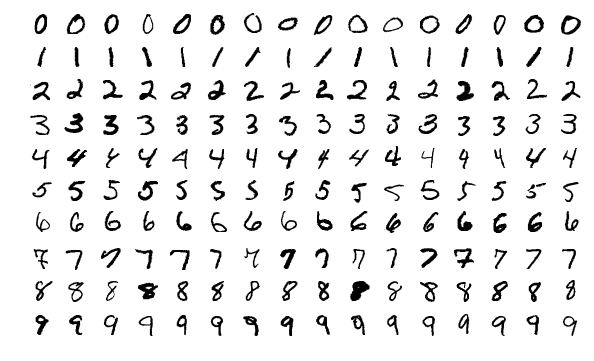
\includegraphics[width=0.7\textwidth]{MnistExamples.png}
        \caption{Samples aus der MNIST-Datenbank~(\cite{lecun2010mnist}):\\
        Erkennung handschriftlicher Ziffern}
    \end{figure}
\end{frame}

\begin{frame}{Beispiele der Bildklassifizierung}
    \begin{figure}
        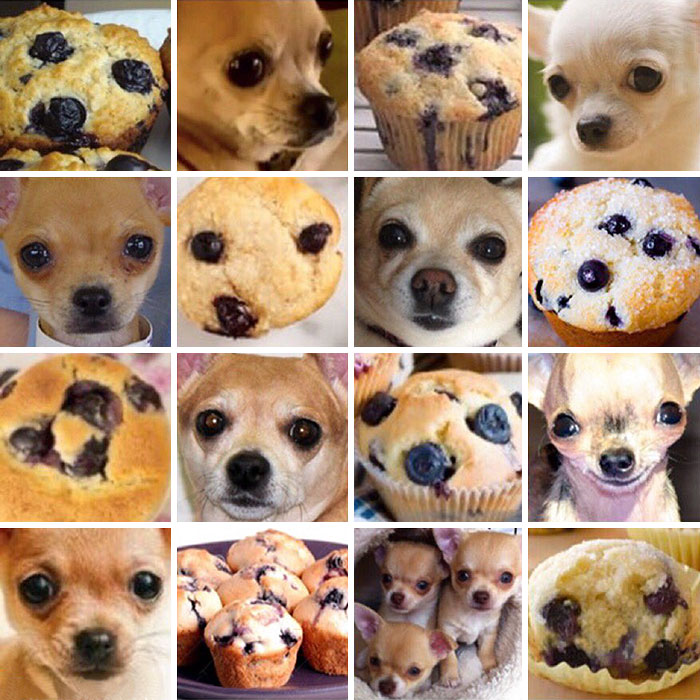
\includegraphics[width=.5\textwidth]{chihuahua.jpg}
        \caption{Chihuahua oder Muffin? {\scriptsize (Grafik aus~\cite{chihuahua})}}
    \end{figure}
\end{frame}

\begin{frame}{Beispiele der Bildklassifizierung}
    \begin{figure}
        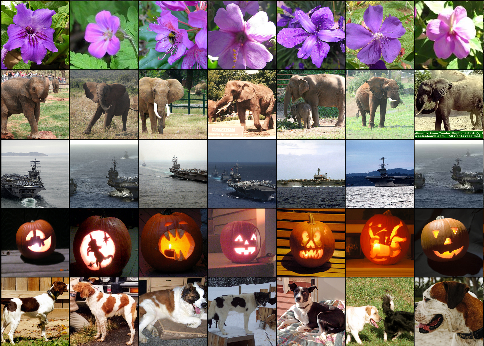
\includegraphics[width=0.7\textwidth]{imagenet-samples.png}
        \caption{Samples aus der ImageNet Large Scale Visual Recognition Challenge 2010 (\cite{ILSVRC15}):\\ Einordnung von Bildern in $1.000$ verschiedene Klassen.
        }
    \end{figure}
\end{frame}


\subsection{Architekturen für Bildklassifizierung}

\begin{frame}{Architekturen für Bildklassifizierung}
    \begin{itemize}
        \item Für die Ziffernerkennung mit $28\times 28$-Pixel Graustufenbildern haben wir bereits ein simples Multi-Layer-Perzeptron als Klassifizierungsnetzwerk kennengelernt.
        \pause\item Dies ist anfällig für Overfitting und für höher aufgelöste, farbige Bildern rechenaufwändig.
        \pause\item \emph{Faltungsnetze} (engl. \foreignlanguage{english}{Convolutional Neural Networks}) setzen stattdessen Faltungslayer ein, um gezielt Merkmale aus den Input-Daten zu extrahieren.
        Mit Poolinglayer wird die Dimension ausreichend reduziert, um mit wenigen Fully-Connected-Layern die Ausgabe zu berechnen.
    \end{itemize}

    \begin{figure}
        \newcommand{\svgwidth}{0.8\textwidth}
        {\scriptsize
        \input{cnn.pdf_tex}
        }
        \caption{Beispielhaftes Faltungsnetz
        {\scriptsize (Grafik angepasst aus \cite{Calin2020})}}
    \end{figure}
\end{frame}

\begin{frame}{LeNet-5}
\begin{figure}
        \newcommand{\svgwidth}{\textwidth}
        {\scriptsize
    \begin{tikzpicture}[main/.style = {draw, outer sep=3pt}] 
    \node[main] (x0) at (0, 0)  {$x_0$}; 
    \node[main] (x1) at (0, -1) {$x_1$};
    \node[main] (x2) at (0, -2) {$x_2$}; 
    \node[main] (x3) at (0, -3) {$x_3$};
    \node[main] (x4) at (0, -4) {$x_4$}; 
    \node[main] (x5) at (0, -5) {$x_5$};

    \node (y0) at (2, -0.5) {$\sigma$};
    \node (y1) at (2, -1.5) {$\sigma$};
    \node (y2) at (2, -2.5) {$\sigma$};
    \node (y3) at (2, -3.5) {$\sigma$};
    \node (y4) at (2, -4.5) {$\sigma$};

    \node[main] (yy0) at (3, -0.5) {$y_0$};
    \node[main] (yy1) at (3, -1.5) {$y_1$};
    \node[main] (yy2) at (3, -2.5) {$y_2$};
    \node[main] (yy3) at (3, -3.5) {$y_3$};
    \node[main] (yy4) at (3, -4.5) {$y_4$};

    \draw [->] (x0) -> node[above, align=center] {$w_0$} (y0);
    \draw [->] (x1) -> node[above, align=center] {$w_1$} (y0);
    \draw [->, gray] (y0) + (0,0.5) -> node[above=3pt, align=center, black] {$b$} (y0);
    \draw [->] (y0) -> (yy0);

    \draw [->] (x1) -> node[above, align=center] {$w_0$} (y1);
    \draw [->] (x2) -> node[above, align=center] {$w_1$} (y1);
    \draw [->, gray] (y1) + (0,0.5) -> node[above=1pt, align=center] {} (y1);
    \draw [->] (y1) -> (yy1);


    \draw [->] (x2) -> node[above, align=center] {$w_0$} (y2);
    \draw [->] (x3) -> node[above, align=center] {$w_1$} (y2);
    \draw [->, gray] (y2) + (0,0.5) -> node[above=1pt, align=center] {} (y2);
    \draw [->] (y2) -> (yy2);


    \draw [->] (x3) -> node[above, align=center] {$w_0$} (y3);
    \draw [->] (x4) -> node[above, align=center] {$w_1$} (y3);
    \draw [->, gray] (y3) + (0,0.5) -> node[above=1pt, align=center] {} (y3);
    \draw [->] (y3) -> (yy3);


    \draw [->] (x4) -> node[above, align=center] {$w_0$} (y4);
    \draw [->] (x5) -> node[above, align=center] {$w_1$} (y4);
    \draw [->, gray] (y4) + (0,0.5) -> node[above=1pt, align=center] {} (y4);
    \draw [->] (y4) -> (yy4);

\end{tikzpicture} 

        }
    \caption{Das LeNet-5 von LeCun et al. in~\cite{lecun1998}, angewandt auf die MNIST-Datenbank.\\
    {\scriptsize(Grafik angepasst aus~\cite{lecun1998})}}
\end{figure}

\begin{itemize}
    \item LeNet-5 hat insgesamt $61.706$ trainierbare Parameter.
    \item Wir vergleichen LeNet-5 mit einem Multi-Layer-Perzeptron mit ähnlich vielen Layern und Parametern: \\
    Die Layergrößen betragen $32x32$, $54$, $48$, $48$, $32$, $10$, die  Parameterzahl $62.240$.
\end{itemize}
\end{frame}

\begin{frame}<presentation:0>[noframenumbering]
    \cite{Calin2020}
    \cite{Goodfellow-et-al-2016}
\end{frame}

\begin{noheadline}
\begin{frame}[allowframebreaks]{Literatur}
	\scriptsize
	\bibliography{../literature}
\end{frame}
\end{noheadline}

\end{document}